\section{Architectural Design}

\subsection{Overview}
	Our system will be designed like a classic four tier JEE application like explained in the figure below.
	\begin{figure}[h!]
		\centering
		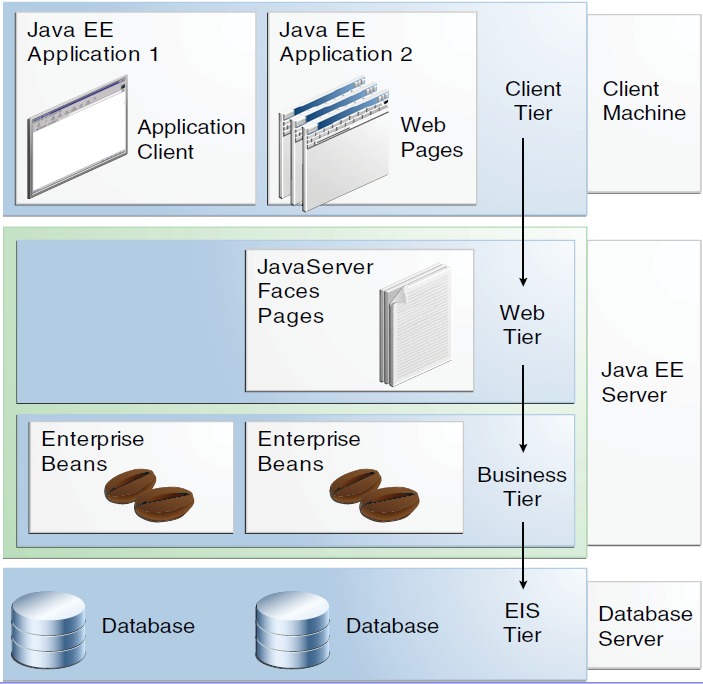
\includegraphics[width=\textwidth]{JEE.png}
	\end{figure}
	
	The client tier contains web pages (while browsing our site through a computer) or a application client (while using the application installed on a smartphone)
	The server tier is dived into two tiers: web tier that is in charge of generating web pages and sending them to the client; and the business tier where all the application's logic is placed. 
	The last tier is the database tier that contains the database server.
		
\subsection{High level components and their interaction}
	This diagram represents the main components of our system and shows how they communicate to each other. On the client side we have only the client component. 
	On the server side we have the ride manager component that will take care of the taxi management side of our application, it will provide an interface to the client. The user manager component will provide functions to manage user account's, this component too will provide an interface to the client, finally the database will hold accounts', taxis' and rides' informations, it will be accessible by the other two server components.
	\begin{figure}[h!]
		\centering
		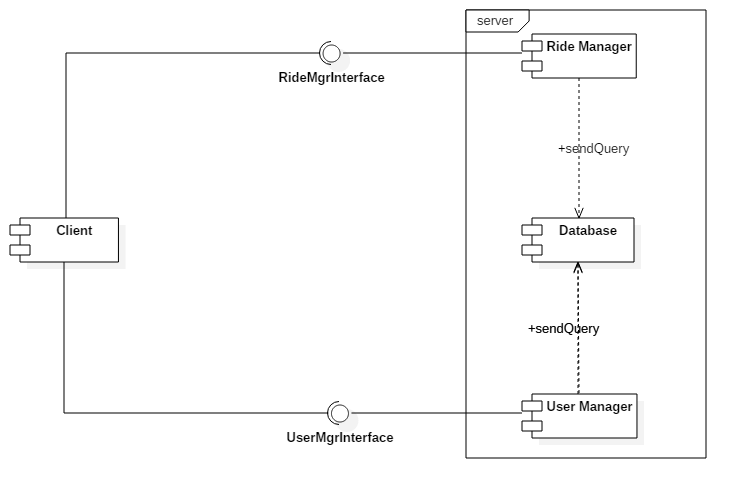
\includegraphics[width=\textwidth]{Component/Model1__high_lvl_comp_1.png}
	\end{figure}
	\newpage
	
\subsection{Component view}
	Here we will provide a more detailed description of the components presented in the previous section.
	\subsubsection{Client component}
	The client is composed by a main component which will have all the basics functions: create account, make request, make reservation; a user interface component that will serve to communicate with the user and finally a connection component that will take care of communicating with the server.
		\begin{figure}[h!]
			\centering
			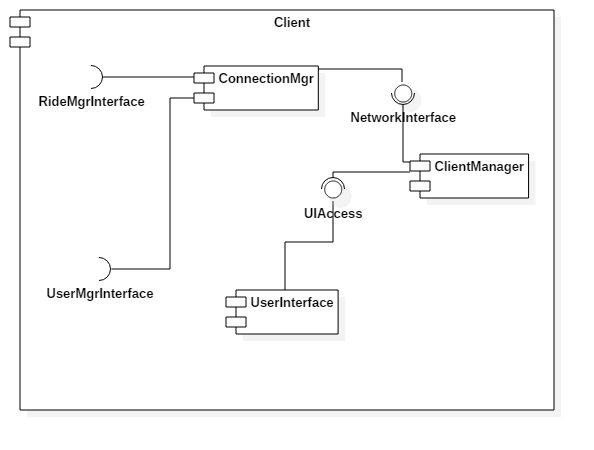
\includegraphics[width=\textwidth]{Component/Model5__client_2.png}
		\end{figure}
		\newpage

	\subsubsection{Ride manager component}
		The ride manager will have a request handler that will take requests or reservation from passengers and forward it to taxi drivers, once a driver has accepted it the ride will be created through the ride generator component. The taxi will be found using the taxi queues manager component. There will be also a connection manager component and a database access component used to access the database.
		The request handler will also take care of join and cancel reservation requests from a passenger. 
		\begin{figure}[h!]
			\centering
			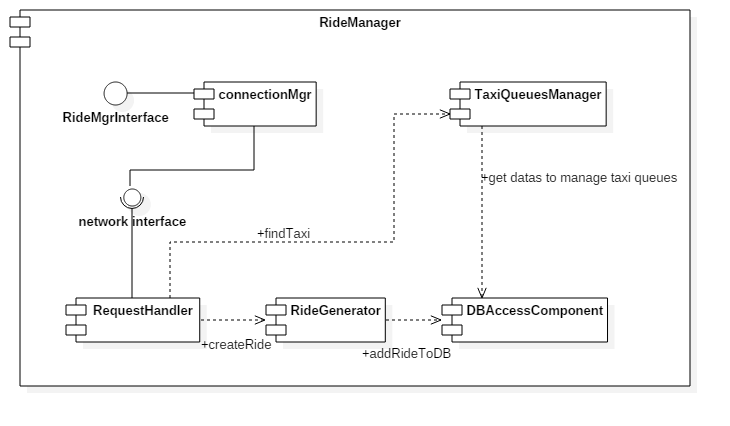
\includegraphics[width=\textwidth]{Component/Model6__ride_mgr_3.png}
		\end{figure}
		\newpage

	\subsubsection{User manager component}
		The user manager will have a account manager component which will provide login and registration functionalities, an account creator component to create new accounts and a database access component.
		\begin{figure}[h!]
			\centering
			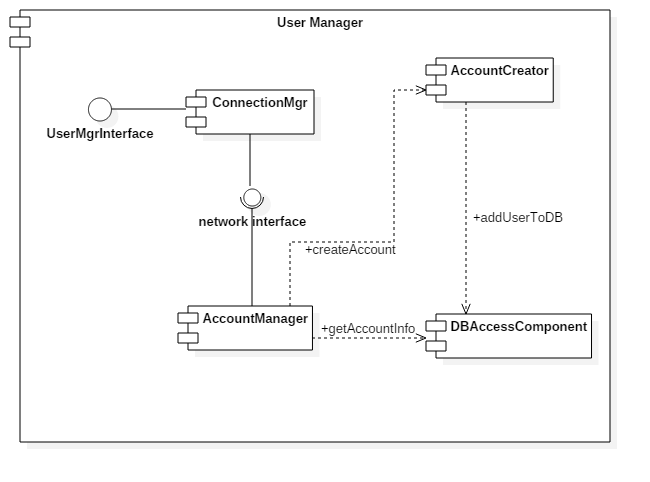
\includegraphics[width=\textwidth]{Component/Model7__user_mgr_4.png}
		\end{figure}
		\newpage
	
	\subsubsection{Database}
	\begin{figure}[h!]
		\centering
%		\includegraphics[width=\textwidth]{ER.png}
	\end{figure}
	\newpage		

\subsection{Deployment view}
This diagram shows how the whole system will be deployed.
The client communicates via HTTPS to the web server and the application server (both web and application servers are installed in the same machine), the web server is responsible to generate web pages, the application server contains all the user and taxi management application's logic and in the end the database.
	\begin{figure}[h!]
		\centering
		\includegraphics[width=\textwidth]{Deployment/deployment.png}
	\end{figure}
	\newpage

\subsection{Runtime view}
	\subsubsection{Login}
	\begin{figure}[h!]
		\centering
		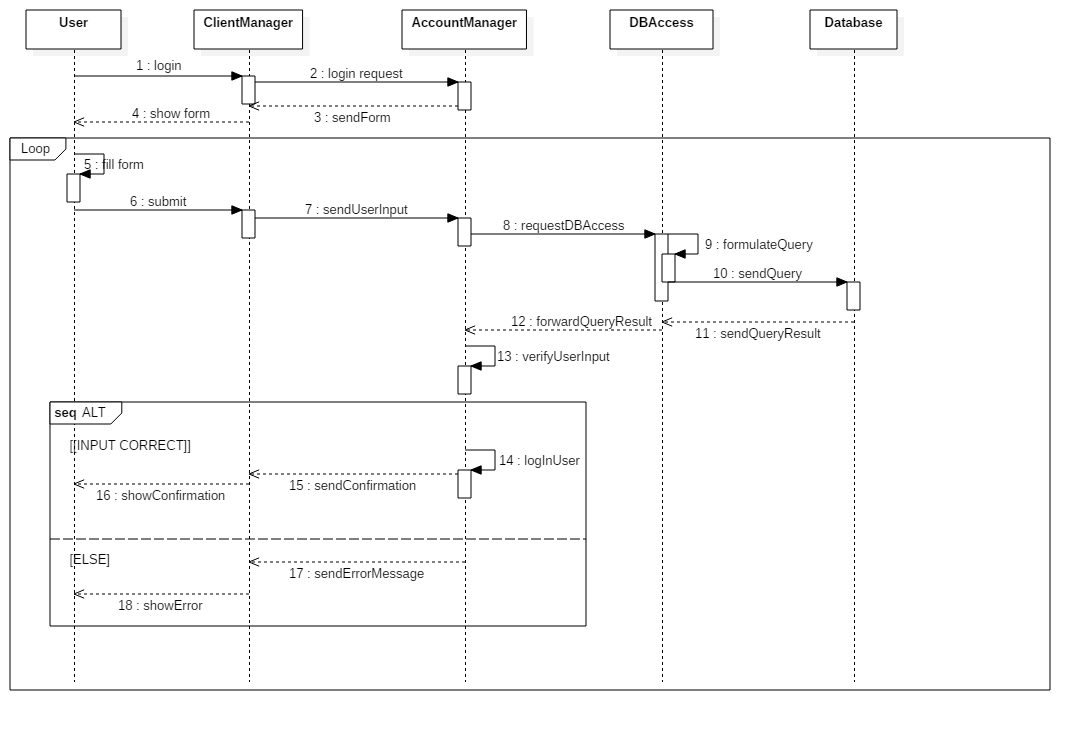
\includegraphics[width=\textwidth]{Sequence/login.png}
	\end{figure}
	\newpage
	
	\subsubsection{Registration}
	\begin{figure}[h!]
		\centering
		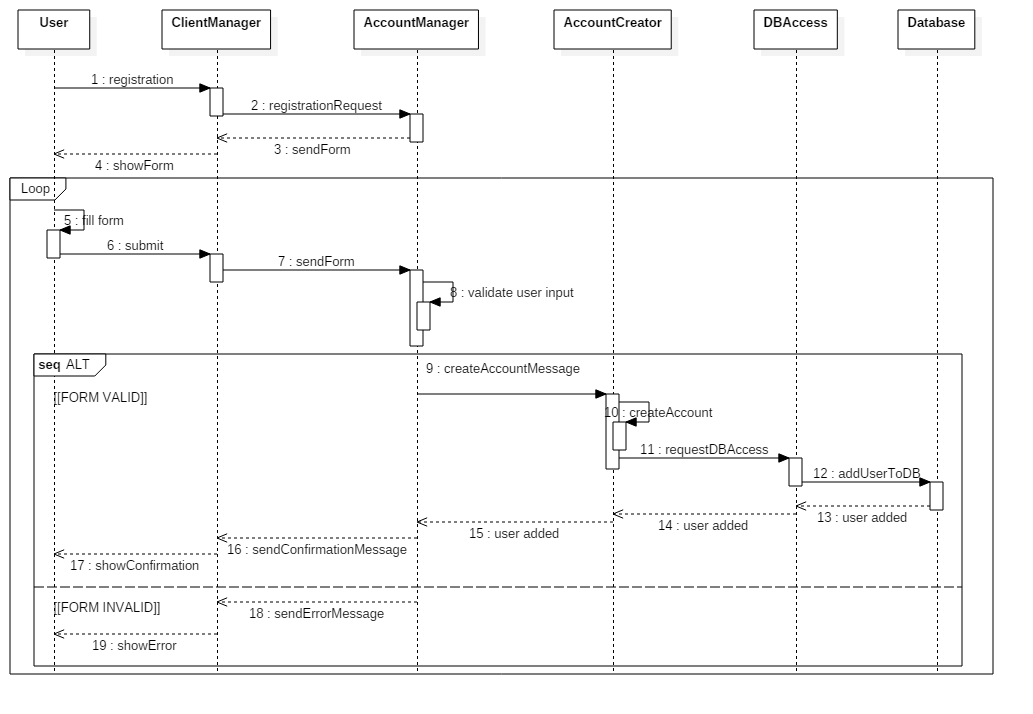
\includegraphics[width=\textwidth]{Sequence/registration.png}
	\end{figure}
	\newpage
	
	\subsubsection{Taxi request}
	\begin{figure}[h!]
		\centering
		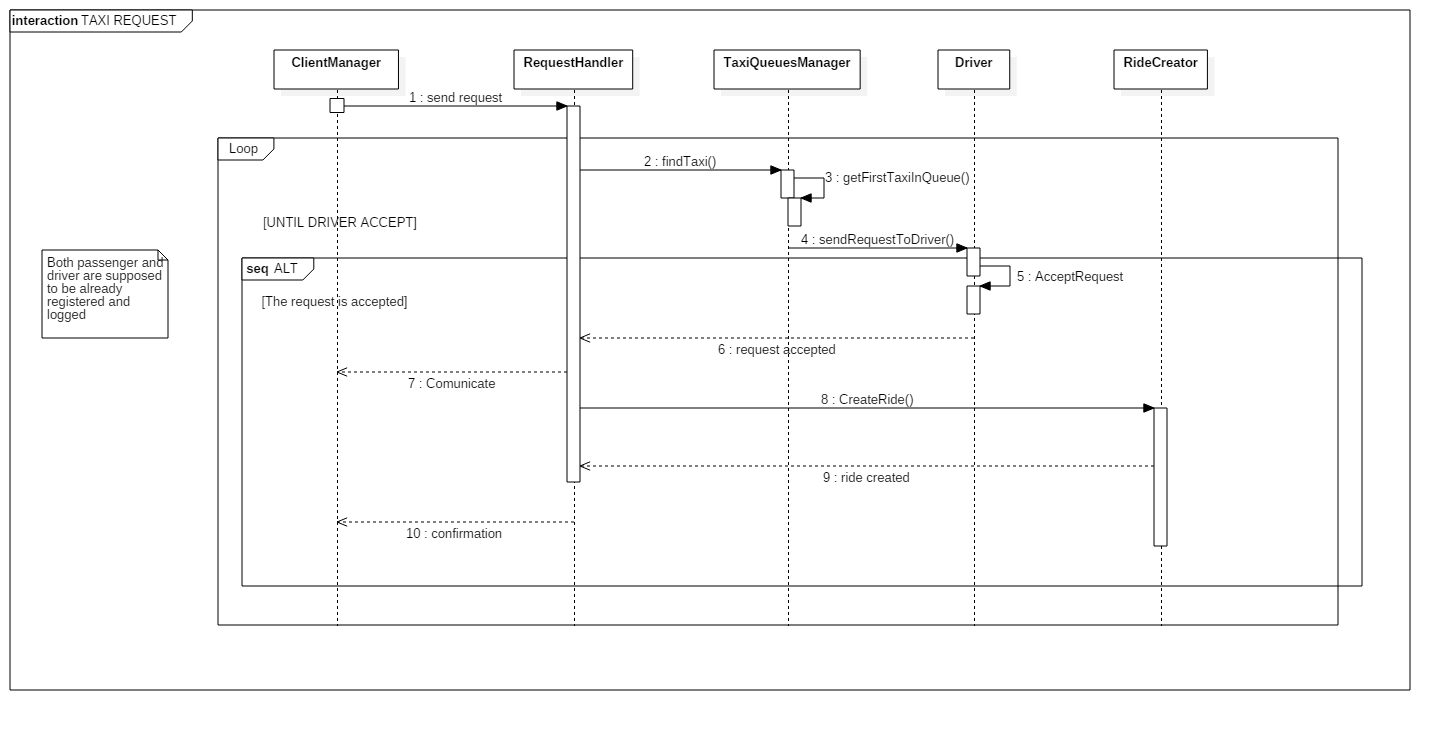
\includegraphics[width=\textwidth]{Sequence/request.png}
	\end{figure}
	\newpage
	
	\subsubsection{Join ride}
	\begin{figure}[h!]
		\centering
		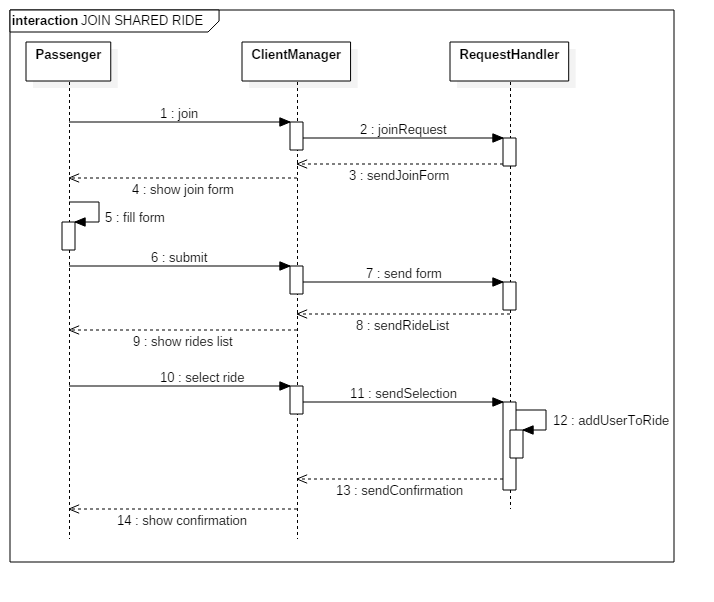
\includegraphics[width=\textwidth]{Sequence/join.png}
	\end{figure}
	\newpage		

	\subsubsection{Accept request}
	\begin{figure}[h!]
		\centering
		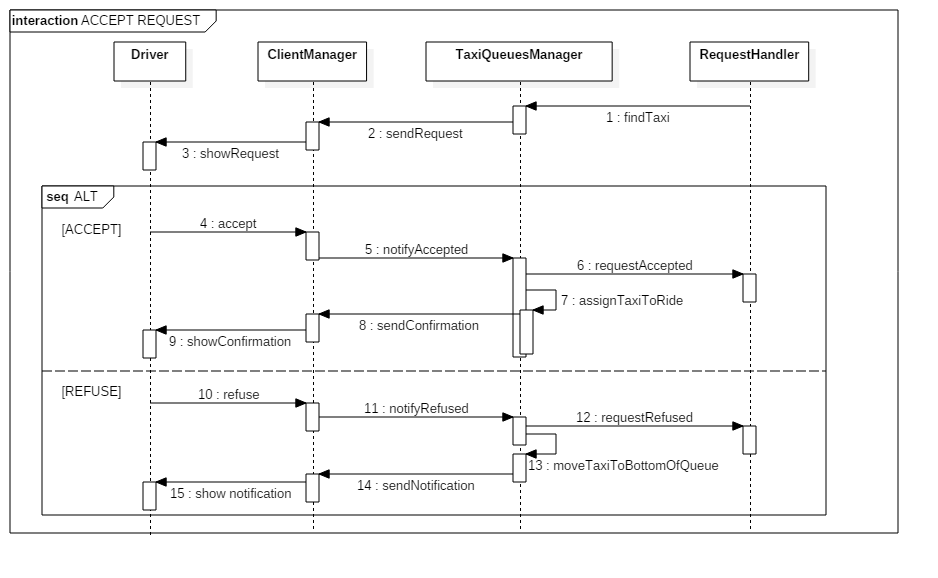
\includegraphics[width=\textwidth]{Sequence/accept_request.png}
	\end{figure}
	\newpage		


\subsection{Component interfaces}
In this section we provide a detailed description of the interfaces we use.

The network interface is used in all the three components, and it's a interface used to provide methods to send and receive user inputs, server's responses and data.
\subsubsection{Client interfaces}
\begin{enumerate}
	\item \textbf{UIAccess}: This interface provides methods to get user input through the user interface
\end{enumerate}
\subsubsection{User Manager interfaces}
\begin{enumerate}
	\item \textbf{Ride Manager interface}: This interface provides to the client methods used to request services from the server, for example for calling a taxi.
\end{enumerate}
\subsubsection{Ride Manager interfaces}
	\begin{enumerate}
		\item \textbf{User Manager interface}: This interface provides to the client methods used to request services from the server such as login and registration requests.
	\end{enumerate}
	
\subsection{Selected architectural styles and patterns}
%credo mvc e cose

\subsection{Other design decisions}